\documentclass{report}
\usepackage{fancyhdr} % Required for custom headers
\usepackage{lastpage} % Required to determine the last page for the footer
\usepackage{extramarks} % Required for headers and footers
\usepackage{graphicx} % Required to insert images

\usepackage{amsmath}
\usepackage{graphicx} 
\usepackage{float}
%\usepackage{amsfont}
%\usepackage{amssymb}

\usepackage{multicol}
% Margins
\topmargin=-0.5in
\evensidemargin=0in
\oddsidemargin=-0.5in
\textwidth=7.5in
\textheight=9.0in
\headsep=0.25in 


\pagestyle{fancy}

%\rhead{\textbf{Marshall's Recipes}} % Top right header
%\lhead{\textbf{Curry Stir Fry}}
%\chead{ }
%\title{Curry Stir Fry}

\begin{document}
%\vspace{8mm}
%\textbf{PRELIMINARIES:}


\bigskip

\bigskip

\begin{multicols}{2}
\textbf{Ingredients}
\begin{itemize}
\item 3 packages ramen noodles (without flavoring) \newline (1140 kCal / 24 gP / 42 gF / 156 gC)
\item 2 tbsp sesame oil \quad (240 kCal / 0 gP / 28 gF / 0 gC)
\item 4 tbsp oyster sauce (60 kCal/ 0 gP/ 0 gF/ 16 gC)
\item 4 tbsp soy sauce \quad (36 kCal / 4 gP / 0 gF / 4 gC)
\item 1 can bean sprouts \quad (35 kCal / 10 gP / 0 gF / 20 gC)
\item 1 tbsp rice vinegar 
\item 1 tsp grated ginger
\item 4-6 green onions, sliced
\item $\frac{1}{2}$ to 1 tbsp chili paste 
\item 6 cloves of garlic
\item 2 lbs asparagus \quad (170 kCal / 44 gP / 0 gF / 68 gC)
\item 6 tbsp. butter  \quad (612 kCal / 0 gP / 24 gF /  gC)
\item 6 eggs (scrambled) \quad (312 kCal / 24 gP / 20 gF / 4 gC) 




\end{itemize}


\columnbreak
\textbf{Procedure:}
\medskip


\begin{enumerate}

\item Prepare the asparagus to sautee and crack eggs into a large bowl.
\item Boil water for ramen. 
\item Scramble eggs and cook in pan with 4 tbsp of butter. Place asparagus in a large pan with 2 tbsp butter on medium-low heat with salt and pepper. 
\item Place ramen in water to boil and whisk together soy sauce, oyster sauce, chili paste, garlic, ginger, and rice vinegar in a bowl. 
\item Drain ramen and place in pot with the sauce mixture and bean sprouts. Stir thoroughly and add scrambled eggs. 
\item Serve with green onion on top and garnish with toasted sesame seeds. 



\begin{table}[H]
  \begin{center}
    \caption{Macro totals}
    \label{tab:table1}
    \begin{tabular}{c|c|c|c} % <-- Alignments: 1st column left, 2nd middle and 3rd right, with vertical lines in between
      \textbf{Calories} & \textbf{Protein} & \textbf{Fat} & \textbf{Carbs}\\
      \hline
      2605 kCal & 212 g & 114 g & 268 g\\
    \end{tabular}
  \end{center}
\end{table}
 
\end{enumerate}
\end{multicols}




%\begin{center}
%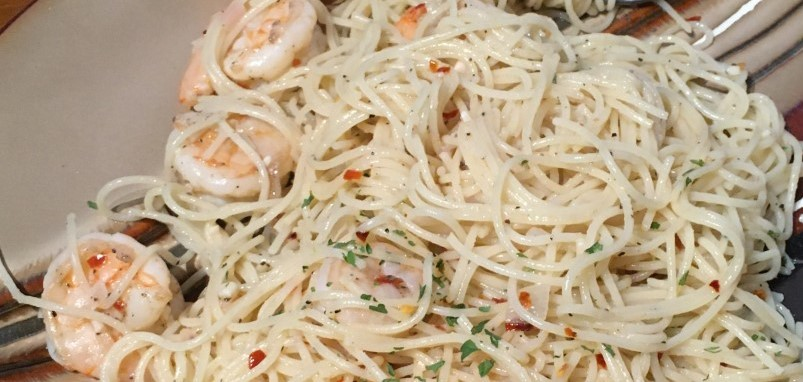
\includegraphics[scale=0.65]{Pasta/Shrimp Scampi/Shrimp Scampi.jpg}
%\end{center}


\end{document}